\section{Installationshandbuch}
In diesem Abschnitt wird die Installation von den einzelnen Komponeneten
ausführlich erklärt, damit die Software, nach dem Herunterladen der questMe repository, erfolgreich gestartet werden kann.

\subsection{Erste Schritte um die Software zum Laufen zu bringen}
Hier werden die ersten Schritte erklärt, die ein Benutzer haben sollte um die
Software ohne Probleme ausführen zu können.

\subsubsection{Setup to run a Angular project}
Hier werden die ersten Schritte für das Einrichten von Angular vorgestellt.
Bei mehr Fragen kann man auch auf das Angular Doc Setup zugreifen,\href{https://angular.io/guide/setup-local}{https://angular.io/guide/setup-local}.
\begin{figure}[H]
    \centering
    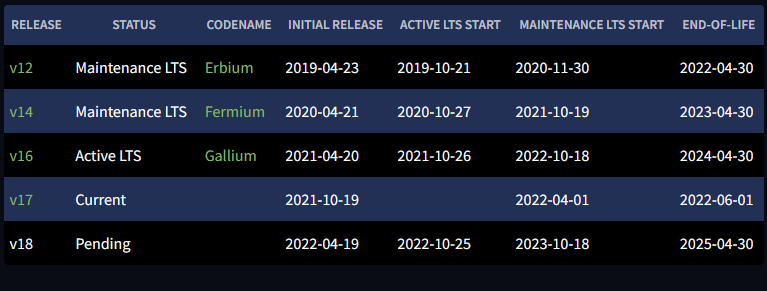
\includegraphics[width=1.0\textwidth]{bilder/installationshandbuch/node.js_version_16.13.0_LTS.PNG}
    \caption{node.js 16.13.0 LTS}
    \label{fig:node.js_16.13.0_LTS}
\end{figure}
\noindent Die node.js Version die in der Software benutzt wird ist die Long Time Support Version \textbf{16.13.0 LTS}, \href{https://nodejs.org/en/about/releases/}{https://nodejs.org/en/about/releases/}.
Diese sollte der Nutzer auf seinen Rechner installiert haben.
Außerdem sollte auch das npm client installiert sein. Zu prüfen ob diese vorhanden ist,
gibt man in dem Terminal Window \textbf{npm -v} ein.\newline

\noindent Der User sollte auch den Angular CLI installieren mit: 
\textbf{npm install -g @angular/cli}

\subsubsection{Docker Comnpose zum Laufen bringen}
Der Benutzer sollte Docker Desktop installiert haben um die Images zu pullen und den Docker compose zu starten.

\begin{figure}[H]
    \centering
    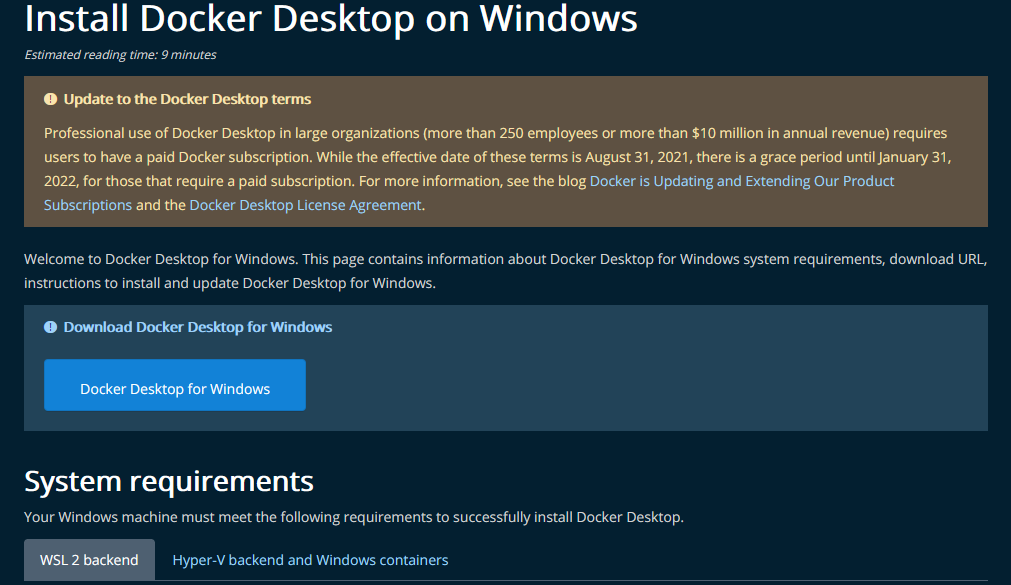
\includegraphics[width=1.0\textwidth]{bilder/installationshandbuch/Docker_Desktop.PNG}
    \caption{Docker Desktop Windows}
    \label{fig:Docker_Desktop_Windows}
\end{figure}
\noindent Wir benutzen bei unserer Software die Windows Version vom Docker Desktop.\newline

\noindent Da wir auf einem Docker arbeiten muss der User nur die Docker Images installieren um den Docker compose zu starten.\newline
Dabei muss er ins Terminal Window und die Images pullen.\newline


\noindent Die Images die der Benutzer pullen sollte.

\begin{itemize}
    \item docker pull mongo:5.0.4-focal
    \item docker pull alpine:3.15
    \item docker pull node:16.13.0-alpine3.14
    \item docker pull openjdk:11
\end{itemize}

\noindent Nachdem die Images gepullt sind kann der Nutzer dann mit \textbf{docker compose build} den docker compose erstellen, indem er es diese 
im Terminal eingibt.\newline

\noindent Um den Docker hochzufahren muss der Benutzer im Terminal \textbf{docker compose up} eingeben.\newline

\noindent Es könnten Schwierigkeiten beim builden entstehen, weil wir den Inhalt der mongoDb im Ordner 
.db-data speichern. 
Um den existierenden Korpus zu löschen muss der Ordner gelöscht werden und das Build erzeugt automatisch eine frisch gefüllte mongoDb mit einem Buildscript beim Starten von mongoDb.

\subsubsection{Docker Desktop mit den Container}
So sollten die Container aussehen und wenn der \textbf{docker compose up} geschieht leuchten die Container grün, wenn nichts 
schief gelaufen ist. Leuchten Sie orange oder rot ist ein Fehler aufgetreten.

\begin{figure}[H]
    \centering
    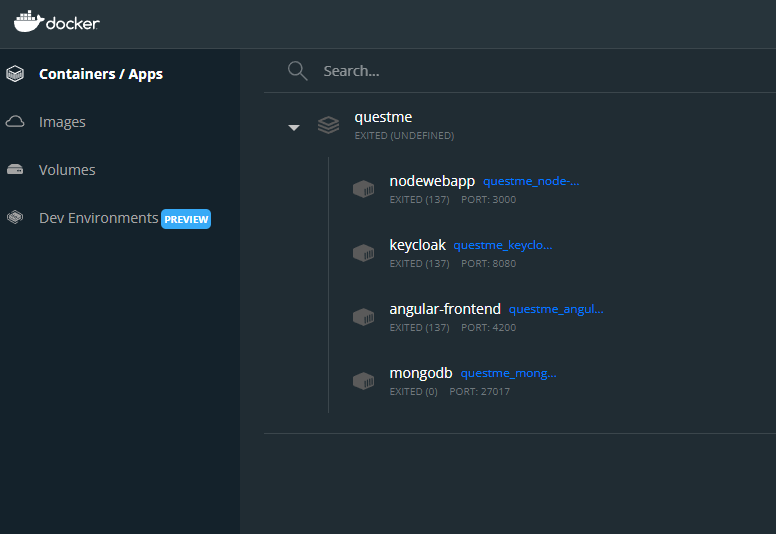
\includegraphics[width=1.0\textwidth]{bilder/installationshandbuch/Docker_Container.PNG}
    \caption{Docker Desktop Container}
    \label{fig:Docker_Desktop_Container}
\end{figure}

